\chapter{Ab Initio Green Kubo: Implementation}
\label{chp:implementation}
\newcommand{\tcut}{t_{\rm c}}

The theoretical background for the \emph{ab initio} simulation of thermal conductivity has been established in the previous chapters, in particular, Chp.~\ref{chp:heat_transport}. The purpose of this chapter is to discuss the practical implementation of the respective formulas. 

We restate the Green-Kubo formula for the thermal conductivity initially introduced in Sec.\,\TODO{ref} as
\begin{align}
	\kappa^{\alpha \beta} (T)
		= \int \d \Gamma_0 ~ \kappa^{\alpha \beta} (\Gamma_0) f_T (\Gamma_0) ~,
	\label{eq:implementation.kappa.avg}
\end{align}
where $\kappa^{\alpha \beta} (T)$ are the Cartesian components of the thermal conductivity tensor at temperature $T$, and $\Gamma_0$ are phase-space configurations with a respective ensemble weight $f_T (\Gamma_0)$ at the given temperature. For each phase-space configuration $\Gamma_0$, the thermal conductivity is computed as
\begin{align}
	\kappa^{\alpha \beta} (\Gamma_0)
		&=
		\frac{V}{k_{\rm B} T^2} 
		\lim_{t_{\rm c} \to \infty}
		\int_{0}^{\tcut} 
		\d t ~ C_{JJ}^{\alpha \beta} (\Gamma_0, t)~,
	\label{eq:implementatino.kappa.1}
\end{align}
where $	C^{\alpha \beta}_{J J} (\Gamma_0, t)$ denotes the heat flux autocorrelation function (HFACF),
\begin{align}
	C^{\alpha \beta}_{J J} (\Gamma_0, t)
		=
		\lim_{t_{0} \to \infty}
		\frac{1}{t_0 - t}
		\int_{0}^{t_{\rm 0} - t} 
		\d s ~ J^\alpha (\Gamma_{t + s}) J^\beta (\Gamma_s)~,
	\label{eq:implementatino.acf.1}
\end{align}
and a phase-space point $\Gamma_t$ is related to the initial configuration $\Gamma_0$ through the canonical time evolution determined by the many-body Hamiltonian of the system, $\mathcal H (\Gamma)$. Equation~\ref{eq:implementation.kappa.avg} through~\ref{eq:implementatino.acf.1} represent an exact reformulation of the Green Kubo formula.


\newthought{In order to evaluate these equations in finite simulations}, the integrals need to be discretized and truncated to finite domains. First, we approximate Eq.\,\eqref{eq:implementation.kappa.avg} by choosing a finite set of starting configurations $\Gamma_0^i$, so that
\begin{align}
	\kappa^{\alpha \beta} (T)
		\approx
		\frac{1}{N} \sum_{i=1}^N \kappa^{\alpha \beta} (\Gamma_0^i)~,
	\label{eq:implementation.kappa.ensemble.approx}
\end{align}
where the starting conditions $\Gamma_0^i$ are chosen from NVT molecular dynamics simulations for the thermodynamic conditions of interest. For each starting condition $\Gamma_0$, we perform NVE molecular dynamics simulations to generate the time evolution of the system, $\Gamma_t$, and evaluate the heat flux, $J^\alpha (\Gamma_t)$ along this trajectory. The simulation is performed for a total simulation time $t_0$, thereby truncating the time integral in Eq.\,\eqref{eq:implementatino.acf.1}. From resulting autocorrelation function of finite length, the thermal conductivity is computed via Eq.\,\eqref{eq:implementatino.kappa.1}, where a \emph{cutoff time} $\tcut < t_0$ is chosen to reduce noise when the autocorrelation function has effectively decayed~\cite{Jones2012}.
After computing the thermal conductivity for each trajectory, the final value is given by Eq.\,\eqref{eq:implementation.kappa.ensemble.approx},~i.\,e.,~by the \emph{mean} of the individual trajectories. The statistical error due to the finite ensemble average is estimated by the \emph{standard error},~i.\,e.,~the standard deviation of the mean,
\begin{align}
	\Delta \kappa^{\alpha \beta} (T)
		= \frac{1}{\sqrt{N}} \sqrt{\frac{1}{N} \sum_i \left( \kappa^{\alpha \beta} (T) - \kappa^{\alpha \beta} (\Gamma_0^i) \right)^2}~.
	\label{eq:imp.delta.kappa}
\end{align}




\newthought{In empirical force field approaches}, the appearing equations are typically evaluated as is, and convergence in size and time can be checked in a brute-force way by increasing the respective scales well beyond the necessary limits\CITE{Lammps, Jones, more}. From an \emph{ab initio} perspective, the accessible size and time scales are each at least two orders of magnitude lower,\footnote{Force fields: 1\,ns for 10000~atoms within 1 day, \emph{ab initio}: 50\,ps for 200~atoms within 1~months.} and additional steps are necessary to increase the amount of information that can be extracted from the comparatively short simulations. The purpose of this chapter is to discuss these additional steps in detail: First, we present steps to remove noise from the heat flux autocorrelation functions $C_{JJ} (t)$, which enables to choose cutoff times $\tcut$ in a numerically robust way. Next, we discuss the size extrapolation scheme in terms of the harmonic mapping presented in Sec.\,\ref{sec:aiGK} which allows to correct for the finite size of simulations cells used in \emph{ab initio} molecular dynamics simulations. Finally, we discuss the necessary simulation times $t_0$ and how those can be estimated for novel materials.

\section{Noise Reduction Scheme}
\subsection{Discard non-contributing terms}
The raw \emph{ab initio} heat flux used in this work was defined in Eq.\,\eqref{eq:J_ai} and is given for a phase-space point $\Gamma_t = \set{{\bf R} (t), \dot{\bf R} (t)}$ by
\begin{align}
	{\bf J}^{\rm raw} (t) = \sum_I \sigma_I (t)  \dot{\bf R}_I (t)~,
	\label{eq:imp.J.0}
\end{align}
where $\sigma_I (t) \equiv \sigma_I [{\bf R} (t)]$ are atomic virial tensors for the configuration at the given time $t$ as defined in Eq.\,\eqref{eq:hf.sigma_I}, and $\dot{\bf R}_I (t)$ is the velocity of atom $I$ as usual. We split the raw flux in two parts,
\begin{align}
	{\bf J}^{\rm raw} (t)
		= \sum_I \delta \sigma_I (t) \dot{\bf R}_I (t) 
		+ \sum_I \braket{\sigma_I} \dot{\bf R}_I (t)~,
	\label{eq:imp.J.1}
\end{align}
where $\braket{\sigma_I}$ is the average atomic virial, and $\delta \sigma_I (t)$ is the time-dependent part. In the absence of diffusion, the second term is the total time derivative of a bounded vector field, $\sum_I \braket{\sigma_I} \dot{\bf R}_I (t) = \frac{\d}{\d t} \sum_I \braket{\sigma_I} {\bf R}_I (t)$. By means of the gauge invariance principle introduced in Sec.\,\ref{sec:gauge_invariance}, it therefore does not contribute to the time integral in Eq.\,\eqref{eq:implementatino.kappa.1}, and can be discarded before evaluating the heat flux autocorrelation function~\cite{Ercole2016}. We therefore always use the following heat flux expression in the following:
\begin{align}
	{\bf J} (t)
		= \sum_I \delta \sigma_I (t) \dot{\bf R}_I (t)~.
	\label{eq:imp.J}
\end{align}
Depending on the material, discarding the non-contributing part from the raw heat flux reduces the noise in the simulation \emph{massively}, as shown for the case of MgO in the upper panel of Fig.\,\ref{fig:imp.hfacf.kappa.1} (orange curves compared to light blue curves).
\begin{figure}
	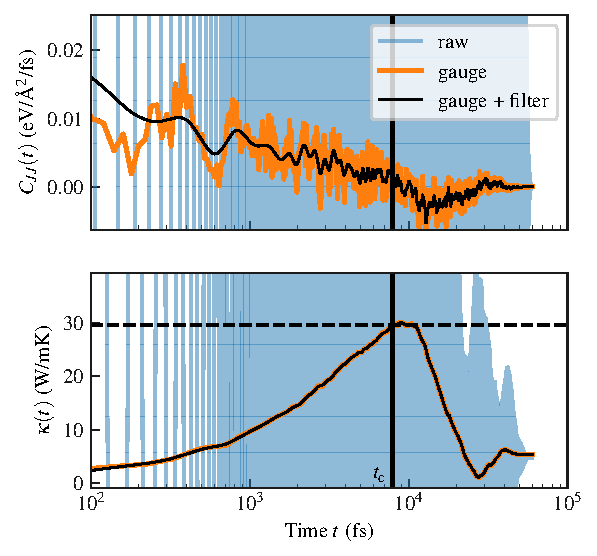
\includegraphics[width=\textwidth]{./data/plots/implementation/MgO/hfacf_data_yy_3.pdf}
	\caption{Heat flux autocorrelation function $C_{JJ}(t)$ (HFACF) as defined in Eq.\,\eqref{eq:implementatino.acf.1} and its cumulative integral,~i.\,e.,~the thermal conductivity $\kappa (t)$ as function of lag time $t$. Light blue: $C_{JJ}(t)$ and $\kappa (t)$ obtained by using the raw flux as defined in Eq.\,\eqref{eq:imp.J.0}. Orange: After discarding the gauge-invariant term in Eq.\,\eqref{eq:imp.J.1}. Black curves: After applying additional, integral-preserving noise filtering as explained in the main text. The cutoff time $t_{\rm c}$ is chosen based on the ``first dip'' of the noise-filtered HFCAF.
	\emph{Computational details:} The shown data is for the $\kappa^{yy}$-component of MgO in an aiMD simulation of 60\,ps total length using a time step of 5\,fs. The heat flux was evaluated every four steps. The system was thermalized to 300\,K using a Langevin thermostat. The system size is 216 atoms in a cubic supercell.}
	\label{fig:imp.hfacf.kappa.1}
\end{figure}

\subsection{Noise filtering}
After discarding the gauge-invariant contributions from the heat flux, there is still a considerable level of noise in the HFACF, which hinders a robust identification of the time at which it is fully decayed,~i.\,e.,~the cutoff time $\tcut$. We investigated several techniques to identify cutoff times, however, most of the available techniques such as the first avalanche technique introduced in Ref.\,\cite{Chen2010} are not fully parameter-free, and need hand tuning, even if very little.\footnote{The first avalanche technique determines cutoff times by means of a signal-over-noise ratio and relies on two parameters, a window size for computing moving averages, and a threshold value for the resulting avalanche function.} We therefore suggest an approach that does only rely on a single parameter which is chosen based on the vibrational spectrum of the material: Motivated by the fact that the \emph{integrated} HFACF,~i.\,e.,~the cumulative thermal conductivity
\begin{align}
	\kappa (t)
		=
		\frac{V}{k_{\rm B} T^2} 
		\int_{0}^{t} 
		\d t' ~ C_{JJ} (t')~,
	\label{eq:imp.kappa.cum}
\end{align}
is already a much smoother function than the HFACF itself, we apply a shape-preserving Savitzky-Golay filter to $\kappa (t)$~\cite{Savitzky1964}. The remaining parameter is the window size for the filter. It is chosen based on the vibrational spectrum of the material by taking the period length corresponding to the slowest significant frequency $\omega_{\min}$. Thereby, all noise of higher frequency is effectively filtered from $\kappa (t)$, while all relevant time integrals are preserved by construction. The filter is constructed such that the antisymmetry of $\kappa (t)$ in time, $\kappa (-t) = - \kappa (t)$ is respected.\footnote{The antisymmetry of $\kappa (t)$ is a consequence of the time symmetry of $C_{JJ} (t)$.} This also ensures that $\kappa (t)$ vanishes identically at $t=0$.

Based on the filtered cumulative thermal conductivity, the HFCAF can be obtained by differentiating, which carries over the filtering to $C_{JJ} (t)$. The filtered HFACF can be obtained analytically by fitting spline functions to $\kappa (t)$, or numerically by applying the same filter on the numerical gradient of $\kappa (t)$. The resulting cumulative thermal conductivity $\kappa (t)$ and HFACF $C_{JJ} (t)$ are shown as black curves in Fig.\,\ref{fig:imp.hfacf.kappa.1}. From the noise-filtered HFACF, the cutoff time $\tcut$ is chosen by a ``first dip'' criterion,~i.\,e.,~when $C_{JJ} (t)$ drops to zero~\CITE{Chen2010 and references therein}. This corresponds to the first significant plateau in $\kappa (t)$ after removing the noise. With the cutoff time $\tcut$, the resulting thermal conductivity for a given component of the thermal conductivity tensor is given by the value $\kappa = \kappa (\tcut)$.

\newthought{The presented scheme} will be used for all reported values of thermal conductivity in the following.

\section{Size extrapolation}
\label{sec:imp.extrapolation}

After we have seen how the Green-Kubo formula is used to compute thermal conductivities from the \emph{ab initio} heat flux evaluated along aiMD trajectories, we shortly review the size extrapolation scheme discussed in more detail in Sec.\,\ref{sec:aiGK}. The aim of the size extrapolation is to correct for finite size effects occuring in aiMD simulations, because the supercells used in \emph{ab initio} simulations are limited in size, and phonon modes of longer wavelength than the supercell are therefore not included. 

\newthought{As discussed in Sec.\,\ref{sec:aiGK}}, the correction works by computing the harmonic contribution to the thermal conductivity $\kappa_{\rm ha}$ within the supercell via Eq.\,\eqref{eq:ha.kappa.bte}
\begin{align}
	\kappa_{\rm ha}^{\alpha \beta} = V k_{\rm B} \sum_{b, {\bf q}} v^\alpha_b ({\bf q}) v^{\beta}_b ({\bf q}) \fD \tau_b ({\bf q})~,
	\label{eq:imp.K.bte}
\end{align}
where $v_b^\alpha ({\bf q})$ is the group velocity of a phonon mode with band index $b$ and \emph{commensurate} wave vector $\bf q$, and $\tau_b ({\bf q})$ is the lifetime obtained from the autocorrelation function of the mode-resolved energy $E_b ({\bf q}, t)$ as defined and discused in Eq.\,\eqref{eq:G_s}~\cite{Carbogno2016}. For a given simulation $\set{\Gamma_t}$, Eq.\,\eqref{eq:imp.K.bte} is evaluated for all commensurate $\bf q$-points, and projected to the symmetry-inequivalent points the Brillouin zone as determinded by the space group operations to improve the statistics~\cite{Maradudin1968,Spglib}.

\newthought{In the next step}, the lifetimes $\tau_b ({\bf q})$ are interpolated to denser $\bf q$-point meshes by $\fD{\tilde{\tau}}_b (\tilde{\bf q}) = \fD \lambda_b (\tilde {\bf q}) \omega_b^{-2} (\tilde {\bf q})$ with a weakly $\bf q$-dependent function $\lambda_b (\tilde {\bf q})$ obtained by linearly interpolating the lifetimes obtained at commensurate $\bf q$-points. The scaling of lifetimes with $\omega_b^{-2} ({\bf q})$ is rooted in basic phonon theory as discussed in detail by Herring~\cite{Herring1954}. For the acoustic modes at ${\bf q} = \Gamma = 0$, where $\omega ({\bf q \to 0}) \to 0$, the value for $\lambda_b (\Gamma)$ is obtained by averaging over values at the surrounding $\bf q$-points. For the new, denser grid, an interpolated value,
\begin{align}
	\kappa_{\rm ha - int}^{\alpha \beta} (N_{\tilde{\bf q}}) = V k_{\rm B} \frac{N_{\bf q}}{N_{\tilde{\bf q}}} \sum_{b, \tilde{\bf q}} v^\alpha_b (\tilde{\bf q}) v^{\beta}_b (\tilde{\bf q}) \fD{\tilde{\tau}}_b (\tilde{\bf q})~,
	\label{eq:imp.K.bte.int}
\end{align}
can be obtained, where $N_{\tilde{\bf q}}$ is the number of points in the new grid, and the factor $N_{\bf q} / N_{\tilde{\bf q}}$ accounts for the increased number points. The bulk limit of Eq.\,\eqref{eq:imp.K.bte.int} is obtained by computing interpolated values for an increasing density of $\bf q$-points. Since Eq.\,\eqref{eq:imp.K.bte.int} is a Riemann sum approximating the Brillouin zone integral $\int \d^3 q$, its convergence can be expected to be linear in $N_{\tilde{\bf q}}^{-1/3} \equiv 1 / n_q$,~i.\,e.,~the inverse number of $\bf q$-points per Cartesian direction. The slope of this curve can be used to extrapolate the value of $\kappa_{\rm ha}$ to bulk limit, as shown in Fig.\,\ref{fig:imp.kappa.bte.int}.
\begin{figure}
	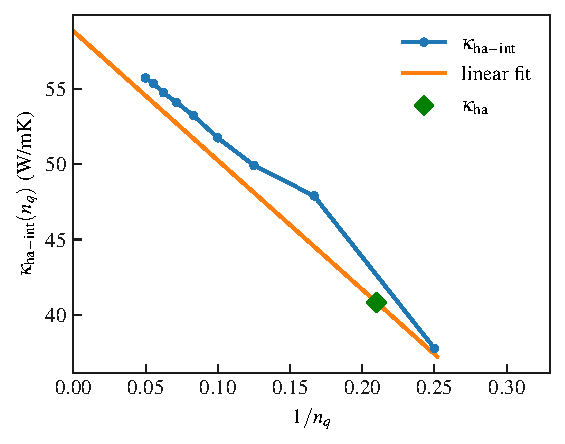
\includegraphics[width=.8\textwidth]{./data/plots/lifetimes/greenkubo_summary_interpolation_fit.pdf}
	\caption{Description of figure}
	\label{fig:imp.kappa.bte.int}
\end{figure}
With the extrapolated value $\kappa_{\rm ha-bulk}$, a correction can be obtained via
\begin{align}
	\delta \kappa_{\rm ha-correction} 
		= \kappa_{\rm ha-bulk} - \kappa_{\rm ha}~,
	\label{eq:imp.K.correction}
\end{align}
from which the final result for the thermal conductivity can be obtained via
\begin{align}
	\kappa^{\alpha \beta}_{\rm corrected}
		 = \kappa^{\alpha \beta} + \delta \kappa^{\alpha \beta}_{\rm ha-correction}~,
	\label{eq:imp.K.corrected}
\end{align}
where $\kappa^{\alpha \beta}$ is the value from the \emph{ab initio} Green Kubo simulation.

